\documentclass{beamer}
\usetheme{A}
\setbeamerfont{frametitle}{size=\normalsize}

\usepackage{amsmath}
\usepackage{datetime}
\usepackage{relsize}
\usepackage{ulem}
\usepackage{amsmath}
\usepackage{calc}
\usepackage{tikz}
\usetikzlibrary{fit,positioning,arrows,automata,shapes,backgrounds,
				calc,patterns}
\tikzset{
	unary/.style={thin,double},
	head/.style={ultra thick}
}
\usepackage{tabularx}
\usepackage{stmaryrd}
\usepackage{wasysym}
\usepackage{booktabs}
\usepackage{multicol}
\usepackage{colortbl}
\usepackage{tabularx}
\usepackage{centernot}
\usepackage{proof}
\usepackage{graphics}
\usepackage{tikz-qtree}
\usepackage{soul}
\usepackage{pifont}

\newcommand{\cmark}{\ding{51}}
\newcommand{\xmark}{\ding{55}}

\usepackage{fontspec}
\newfontfamily\DejaSans{DejaVu Sans}

\definecolor{darkgreen}{HTML}{009900}
\definecolor{darkred}{HTML}{e60000}
\definecolor{darkyellow}{HTML}{ff9900}
\newcommand{\dg}[1]{\textcolor{darkgreen}{#1}}
\newcommand{\dr}[1]{\textcolor{darkred}{#1}}
\newcommand{\dy}[1]{\textcolor{darkyellow}{#1}}
\newcommand{\happy}{\dg{\smiley}}
\newcommand{\sad}{\dr{\frownie}}

\newcolumntype{L}{>{\raggedright\arraybackslash}X}
\newcommand{\hnorm}{\vphantom{()}}

\hypersetup{
    colorlinks=true,
    urlcolor=blue,
    pdfpagemode=FullScreen,
}


%%%%%%%%%%%%%%%%%%%%%%%%%%%%%%%%%%%%%%%%%%%%%%%%%%%%%%%%%%%%%%%%%%%%
%                  term / type / rule macros
\newcommand{\lam}{\mathnormal{\lambda}}
\newcommand{\smallprop}[1]{\ensuremath{\normalfont\textsc{#1}}}
\newcommand{\prop}[1]{\ensuremath{\vnorm{\smallprop{#1}}}}
\newcommand{\smallterm}[1]{\ensuremath{\mathsf{#1}}}
\newcommand{\term}[1]{\smallterm{#1}}
\newcommand{\propcon}{\ensuremath{\mathsf{Prop}_0}}
\newcommand{\cterm}[1]{\textrm{#1}}
\newcommand{\li}{\scalebox{1}[1]{\ensuremath{\multimap}}}
\newcommand{\ii}{\scalebox{1}[1]{\ensuremath{\to}}}
\newcommand{\il}{\scalebox{-1}[1]{$\li$}}
\newcommand{\divleft}{\backslash}
\newcommand{\divright}{	/}
\newcommand{\with}{{\ensuremath{\&}}}
\newcommand{\rulestyle}[1]{\ensuremath{\mathrm{#1}}}
\newcommand{\Exchange}{\rulestyle{ex}}
\newcommand{\Contraction}{\rulestyle{contr}}
\newcommand{\Weakening}{\rulestyle{weak}}
\newcommand{\Extraction}{\ensuremath{\rulestyle{extr}_{\xdiamond}}}
\newcommand{\Lex}{\rulestyle{lex}}
\newcommand{\Ax}{\rulestyle{id}}
\newcommand{\ctx}[1]{\llbracket{#1}\rrbracket}
\newcommand{\bracket}[1]{\langle{#1}\rangle}
\newcommand{\appright}{\ensuremath{\triangleleft}}
\newcommand{\appleft}{\ensuremath{\triangleright}}
\newcommand{\nappright}{\ensuremath{\blacktriangleleft}}
\newcommand{\nappleft}{\ensuremath{\blacktriangleright}}
\newcommand{\adbmal}{\scalebox{-1}[1]{\ensuremath{\lambda}}}
\newcommand{\types}{\ensuremath{\mathcal{U}}}
\newcommand{\lexicon}{\ensuremath{\mathcal{L}}}
\newcommand{\terms}{\ensuremath{\smallterm{Terms}}}
\newcommand{\cons}{\ensuremath{\smallterm{Cons}}}
\newcommand{\con}[1]{\smallterm{c}_{\mathnormal{#1}}}
\newcommand{\vars}{\ensuremath{\smallterm{Vars}}}
\newcommand{\str}[1]{\smallterm{\sslash{#1}\sslash}}
\newcommand{\Var}[1]{\smallterm{x}_{\mathnormal{#1}}}
\newcommand{\vari}{\Var{i}}
\newcommand{\varj}{\Var{j}}
\newcommand{\vark}{\Var{k}}
\newcommand{\varl}{\Var{l}}
\newcommand{\varm}{\Var{m}}
\newcommand{\varn}{\Var{n}}
\newcommand{\varo}{\Var{o}}

\newcommand{\ninfer}[3]{\infer[\!\!{#1}]{#2}{#3}}

%%%%%%%%%%%%%%%%%%%%%%%%%%%%%%%%%%%%%%%%%%%%%%%%%%%%%%%%%%%%%%%%%%%
%					grammar shortcuts
\newcommand{\w}[1]{\text{#1}}
\newcommand{\smallgtype}[1]{\ensuremath{#1}}
\newcommand{\gtype}[2][l]{%
	\ifthenelse
		{\equal{#1}{s}}%
		{\smallgtype{#2}}%
		{\ensuremath{\vnorm{\smallgtype{#2}}}}%
}
\newcommand{\subcat}[3]{\ensuremath{\gtype[#1]{#2}_{\text{#3}}}}
\newcommand{\s}[1][]{\gtype[#1]{s}}
\newcommand{\smalls}{\s[s]}
\newcommand{\smain}[1][]{\subcat{#1}{\smalls}{dcl}}
\newcommand{\smallsmain}{\smain[s]}
\newcommand{\svi}[1][]{\subcat{#1}{\s}{vi}}
\newcommand{\smallsvi}{\svi[s]}
\newcommand{\ssub}[1][]{\subcat{#1}{\s}{sub}}
\newcommand{\smallssub}{\ssub[s]}
\newcommand{\np}[1][]{\gtype[#1]{np}}
\newcommand{\smallnp}{\np[s]}
\newcommand{\n}[1][]{\gtype[#1]{n}}
\newcommand{\smalln}{\n[s]}
\newcommand{\pp}[1][]{\gtype[#1]{pp}}
\newcommand{\smallpp}{\pp[s]}
\newcommand{\type}[1][]{\gtype[#1]{Type}}
\newcommand{\base}[1][]{\gtype[#1]{Base}}
%%%%%%%%%%%%%%%%%%%%%%%%%%%%%%%%%%%%%%%%%%%%%%%%%%%%%%%%%%%%%%%%%%%%
%				extraction shortcuts (extra)
\newcommand{\adj}[1][]{\gtype[#1]{adj}}
\newcommand{\bw}[1][]{\gtype[#1]{bw}}
\newcommand{\letter}[1][]{\gtype[#1]{let}}
\newcommand{\punct}[1][]{\gtype[#1]{punct}}
\newcommand{\lid}[1][]{\gtype[#1]{lid}}
\newcommand{\vnw}[1][]{\gtype[#1]{vnw}}
\newcommand{\tsw}[1][]{\gtype[#1]{tsw}}
\newcommand{\tw}[1][]{\gtype[#1]{tw}}
\newcommand{\vg}[1][]{\gtype[#1]{vg}}
\newcommand{\vz}[1][]{\gtype[#1]{vz}}
\newcommand{\ww}[1][]{\gtype[#1]{ww}}
\newcommand{\adv}[1][]{\gtype[#1]{adv}}
\newcommand{\ahi}[1][]{\gtype[#1]{ahi}}
\newcommand{\adjp}[1][]{\gtype[#1]{adjp}}
\newcommand{\cp}[1][]{\gtype[#1]{cp}}
\newcommand{\detp}[1][]{\gtype[#1]{detp}}
\newcommand{\infp}[1][]{\gtype[#1]{inf}}
\newcommand{\oti}[1][]{\gtype[#1]{oti}}
\newcommand{\ti}[1][]{\gtype[#1]{ti}}
\newcommand{\ppart}[1][]{\gtype[#1]{ppart}}
\newcommand{\ppres}[1][]{\gtype[#1]{ppres}}
\newcommand{\rel}[1][]{\gtype[#1]{rel}}
\newcommand{\svan}[1][]{\subcat{#1}{\smalls}{van}}
\newcommand{\wh}[1][]{\gtype[#1]{wh}}
\newcommand{\sub}[1][]{\gtype[#1]{sub}}
\newcommand{\whq}[1][]{\subcat{#1}{\wh[s]}{q}}
\newcommand{\whrel}[1][]{\subcat{#1}{\wh[s]}{rel}}
\newcommand{\whsub}[1][]{\subcat{#1}{\wh[s]}{sub}}

%%%%%%%%%%%%%%%%%%%%%%%%%%%%%%%%%%%%%%%%%%%%%%%%%%%%%%%%%%%%%%%%%%%%
%					type modalities

\makeatletter
\newcommand{\getfontdim}[1]{%
  \fontdimen22
  \ifx#1\displaystyle\textfont\else
  \ifx#1\textstyle\textfont\else
  \ifx#1\scriptstyle\scriptfont\else
  \scriptscriptfont\fi\fi\fi 2
}
\makeatother

\newcommand{\dgat}[2]{\alt<#1>{\dg{#2}}{#2}}
\newcommand{\drat}[2]{\alt<#1>{\dr{#2}}{#2}}
\newcommand{\boxat}[2]{\ensuremath{\alt<#1>{\boxed{#2}}{#2}}}
\newcommand{\qmarkat}[2]{\alt<#1>{#2}{???}}
\newcommand{\gqmarkat}[2]{\dg{\alt<#1>{#2}{???}}}
\newcommand{\rqmarkat}[2]{\dr{\alt<#1>{#2}{???}}}

% ratio: 1.8/2.75
\newcommand{\domodaldiamondscale}[2]{\raisebox{0.175\getfontdim{#1}}{\scalebox{0.9}{\ensuremath{#1#2}}}}
\newcommand{\domodalboxscale}[2]{\raisebox{0.15\getfontdim{#1}}{\scalebox{0.85}{\ensuremath{#1#2}}}}
\newcommand{\domodalxdiascale}[2]{\raisebox{0\getfontdim{#1}}{\scalebox{1.375}{\ensuremath{#1#2}}}}
\newcommand{\modalxdiascale}[1]{\mathpalette\domodalxdiascale{#1}\relax}
\newcommand{\modaldiamondscale}[1]{\mathpalette\domodaldiamondscale{#1}\relax}
\newcommand{\modalboxscale}[1]{\mathpalette\domodalboxscale{#1}\relax}
\renewcommand{\diamond}{\modaldiamondscale{\diamondsuit}}
\newcommand{\xdiamond}{\modalxdiascale{\vardiamondsuit}}
\newcommand{\bx}{\modalboxscale{\Box}}
\newcommand{\xbx}{\modalboxscale{\blacksquare}}
\newcommand{\dep}[1]{\ensuremath{{\smaller #1}}}
\newcommand{\deps}{\ensuremath{\mathsf{Deps}}}
\newcommand{\adjuncts}{\ensuremath{\dep{Adjs}}}
\newcommand{\complements}{\ensuremath{\dep{Comps}}}
\newcommand{\ddia}[1]{\diamond_{\scalebox{0.66}{\dep{\smaller{#1}}}}}
\newcommand{\dxdia}[1]{\xdiamond_{\scalebox{0.66}{\dep{\smaller{#1}}}}}
\newcommand{\dbox}[1]{\bx_{\scalebox{0.66}{\dep{\smaller{#1}}}}}
\newcommand{\dxbox}[1]{\xbx_{\scalebox{0.66}{\dep{\smaller{#1}}}}}
\newcommand{\dbra}[2]{\bracket{#1}^{\scalebox{0.66}{\dep{#2}}}}

%%%%%%%%%%%%%%%%%%%%%%%%%%%%%%%%%%%%%%%%%%%%%%%%%%%%%%%%%%%%%%%%%%%%
%                  term modalities
\makeatletter
\newcommand{\domodaltermscale}[2]{\raisebox{0.25\getfontdim{#1}}{\scalebox{0.85}{\ensuremath{#1#2}}}}
\makeatother
\newcommand{\modaltermscale}[1]{\mathpalette\domodaltermscale{#1}\relax}
\newcommand{\boxelim}{\modaltermscale{\blacktriangledown}}
\newcommand{\dboxelim}[1]{\boxelim_\dep{#1}}
\newcommand{\boxintro}{\modaltermscale{\blacktriangle}}
\newcommand{\diaelim}{\modaltermscale{\triangledown}}
\newcommand{\ddiaelim}[1]{\diaelim_\dep{#1}}
\newcommand{\diaintro}{\modaltermscale{\vartriangle}}
\newcommand{\ddiaintro}[1]{\diaintro_\dep{#1}}
\newcommand{\caseof}[3]{\cterm{case \term{#1} of \term{#2} in \term{#3}}}

%%%%%%%%%%%%%%%%%%%%%%%%%%%%%%%%%%%%%%%%%%%%%%%%%%%%%%%%%%%%%%%%%%%%
%					logics
\newcommand{\logic}[1]{\textbf{#1}}
\newcommand{\ILL}{\logic{ILL}}
\newcommand{\IL}{\logic{IL}}
\newcommand{\LC}{\logic{L}}
\newcommand{\NL}{\logic{NL}}
\newcommand{\NLP}{\logic{NLP}}
\newcommand{\LP}{\logic{LP}}
\newcommand{\NLPplus}{\ensuremath{\NLP_{\diamond,\bx}}}
\newcommand{\hm}[1]{\ensuremath{\lceil{#1}\rceil}}

%%%%%%%%%%%%%%%%%%%%%%%%%%%%%%%%%%%%%%%%%%%%%%%%%%%%%%%%%%%%%%%%%%%%
%                  proofnet stuff
\newcommand{\pprop}[1]{\ensuremath{\smallprop{#1}^{+}}}
\newcommand{\nprop}[1]{\ensuremath{\smallprop{#1}^{-}}}
\newcommand{\vnorm}[1]{\vphantom{\dbra{\chi}{cnj}}{#1}}
\newcommand{\parlink}{\raisebox{\depth}{\scalebox{-1}[-1]{$\with$}}}
\newcommand{\sbind}{\ensuremath{\mkern-0.5mu\cdot\mkern-0.5mu }}

\newcommand{\scratchat}[2]{\alt<{#1}>{\st{#2}}{#2}}
%\newcommand{\colorat}[3]{\alt<{#1}>{\textcolor{#2}{#3}}{#3}}


\begin{document}



\date{LSD, Sept 12, G\"oteborg}

\title[]{Geometry-Aware Supertagging}
\subtitle[]{with Heterogeneous Dynamic Convolutions}
\author{%
    Konstantinos Kogkalidis\textsuperscript{1,2} \and \& \and Michael Moortgat\textsuperscript{2}\\ 
    ~\\
	~\inst{1 Aalto University}\\
    ~\inst{2 Utrecht Institute of Linguistics OTS, Utrecht University}
}


{%
\setbeamertemplate{headline}{}
\frame{\titlepage
\hspace{-10pt}
\begin{minipage}{0.5\textwidth}
\begin{minipage}{0.35\textwidth}
\includegraphics[scale=0.065]{NWO logo - RGB_wit_rondom_0.jpg}%
\end{minipage}%
\begin{minipage}{0.65\textwidth}
\smaller[3]
\centering
A composition calculus for vector-based semantic modelling
with a localization for Dutch\\~\\
NWO 360-89-070, 2017-2023
\end{minipage}
\end{minipage}%
\hfill
\begin{minipage}{0.45\textwidth}
\hfill
\raisebox{-5.5pt}{\includegraphics[scale=0.5]{UU_logo_2021_EN_RGB.jpg}}
\end{minipage}%
}
}


\section{Categorial Grammars}

\begin{frame}{Categorial Grammars 101}
    \smaller
    \begin{block}{\textbf{\smaller what are they?}}
    A \textbf{family} of syntactic formalisms; each instance consists of:
        \begin{itemize}
            \item a \textbf{lexicon}\\
            a map assigning \textit{categories} to words:
            (quasi-)logical formulas (or ADTs)
            \item a small set of \textbf{inference rules}\\
            ways to combine and reduce \textit{expressions} based on their categories 
        \end{itemize}
    \end{block}
\end{frame}

\begin{frame}{Categorial Grammars 101}
    \smaller
    \textbf{Many variations}: TLG, ACG, CCG, \dots ({\text{*}}CG)\\
    \hfill
    
    \alt<2->{
        \begin{block}{\smaller \textbf{divergences}}
            different background logics $\implies$
            \begin{itemize}
                \item different linguistic aspects captured\\
                \textit{e.g. surface order, non-local syntax, dependency relations}
                \item different parsing complexity\\
                \item different computational semantics\\
                \item \dots
            \end{itemize}
        \end{block}
        \vfill
    }
    {
        \begin{block}{\smaller \textbf{common points}}
            \begin{itemize}
                \item \textbf{Lexicalized}\\
                words come packed with their combinatorics 
                \item \textbf{Formal}\\
                proximal to logics, type theory \& functional programming
                \item \textbf{Transparent}\\
                neat syntax-semantics interface
            \end{itemize}
        \end{block}
    }
\end{frame}

\begin{frame}{Categorial Grammars 101}
    \smaller
    
    \begin{block}{\smaller{\alert{but!} the \textbf{parsing pipeline} is always the same}}
    given an input sentence:
        \begin{enumerate}
            \item Assign a category to each word
            \item Build the syntactic derivation bottom-up
            \item ???
            \item Profit
        \end{enumerate}
    \end{block}\vfill
    
    \noindent
%    \hfill\makebox[30pt][l]{%
%      \raisebox{0pt}[60pt][0pt]{%
%        \includegraphics[scale=0.2]{Screenshot 2022-05-30 at 20-21-00 Underpants Gnomes.png}}
%    }
    
\end{frame}

\section{Supertagging}


\begin{frame}{Supertagging: the task}
    \smaller
    For some input sentence $w_1, \dots w_n$ find the category assignment $c_1, \dots c_n$ s.t.
        \[
            argmax_{(c_1, \dots c_n)}~ p(c_1, \dots c_n ~ | ~ w_1, \dots w_n)^*
        \]
        
    \vfill
    \visible<2->{
    \begin{flushright}
    \begin{minipage}{0.875\textwidth}
    \smaller
    \textsuperscript{\text{*}}\textit{In practice}:\\
    \textit{build the best statistical model possible given current technology and available data}
    \end{minipage}
    \end{flushright}
    }
\end{frame}

\begin{frame}{(pre-)history}
\smaller
    $
    p(t_1, \dots t_n ~ | ~ w_1, \dots w_n) \approx
    $
    
    \begin{itemize}
        \uncover<2->{
        \item $\prod_i^n (t_i~|~w_i)$\\
        \quad \textit{co-occurrence-based statistical models (90s)}}
        \uncover<3->{
        \item $\prod_i^n (t_i~|~w_{i-\kappa} \dots w_{i+\kappa})$\\
        \quad \textit{window-based n-gram models (00s), FFNs (early 10s)}}
        \uncover<4->{
        \item $\prod_i^n (t_i~|~w_1,\dots w_n)$\\
        \quad \textit{sequence encoders (mid 10s)}}
        \uncover<6->{
        \item $\prod_i^n (t_i~|~t_1, \dots t_{i-1}, w_1,\dots w_n)$\\ 
        \quad \textit{seq2seq (late 10s)}}
    \end{itemize}
    \vfill

	\alt<11->{
what have we done?
\begin{itemize}
        \item[$\bullet$] more arrows (=more context)
        \item[$\bullet$] auto-regression (price: temporal delay)
        \item[$\bullet$] what about the co-domain?	
\end{itemize}
}
{
      \centering
        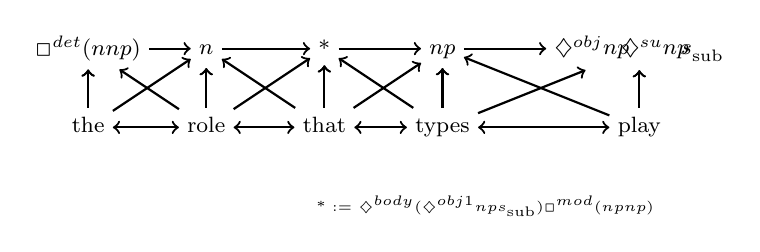
\begin{tikzpicture}
        [ctx/.style={thick, ->},
         ctxbi/.style={thick, <->}]
        	\smaller
        		\node			(w1)				at (-8.5, 0)  	{\hnorm the};
        		\node			(t1)				at (-8.5, 1)		{$\Box^{det} (n \li np)$};
        		\node			(w2)				at (-7,0)		{\hnorm role};
        		\node			(t2)				at (-7, 1)		{\hnorm $n$};
        		\node			(w3)				at (-5.5, 0)		{\hnorm that};
        		\node			(t3)				at (-5.5, 1)		{*};
        		\node			(w4)				at (-4, 0)		{\hnorm types};
        		\node			(t4)				at (-4, 1)		{\hnorm $np$};
        		\node			(w5)				at (-1.5, 0)		{\hnorm play};
        		\node			(t5)				at (-1.5, 1)		{\hnorm $\diamondsuit^{obj}np \!\li\! \diamondsuit^{su} np \! \li \! \ssub$};
        		\node 			(explain)		at (-3.5,-1) 	{\smaller[2] * := $\diamondsuit^{body}(\diamondsuit^{obj1}np\li \ssub)\li \Box^{mod}(np\li np)$};
        		%
        		\visible<2-3,5>{
	        		\draw[ctx] (w1) -- (t1);
        			\draw[ctx] (w2) -- (t2);
	        		\draw[ctx] (w3) -- (t3);
    	    		\draw[ctx] (w4) -- (t4);
        			\draw[ctx] (w5) -- (t5);
        		}
        		\visible<3>{
	        		\draw[ctx] (w2) -- (t1);
	        		\draw[ctx] (w1) -- (t2);
	        		\draw[ctx] (w3) -- (t2);
	        		\draw[ctx] (w2) -- (t3);
	        		\draw[ctx] (w4) -- (t3);
	        		\draw[ctx] (w3) -- (t4);
	        		\draw[ctx] (w5) -- (t4);
	        		\draw[ctx] (w4) -- (t5);
        		}
        		\visible<4->{
        			\draw[ctxbi] (w1) -- (w2);
        			\draw[ctxbi] (w2) -- (w3);
        			\draw[ctxbi] (w3) -- (w4);
        			\draw[ctxbi] (w4) -- (w5);
        		}
        		\visible<6->{
        			\draw[ctx] (w1) -- (t1);
        		}
        		\visible<7->{
        			\draw[ctx] (t1) -- (t2);
        			\draw[ctx] (w2) -- (t2);
				}
				\visible<8->{        			
        			\draw[ctx] (t2) -- (t3);
        			\draw[ctx] (w3) -- (t3);
        		}
        		\visible<9->{
        			\draw[ctx] (t3) -- (t4);
        			\draw[ctx] (w4) -- (t4);
        		}
        		\visible<10->{
        			\draw[ctx] (t4) -- (t5);
        			\draw[ctx] (w5) -- (t5);
        		}
        \end{tikzpicture}
	}
\end{frame}

\begin{frame}{Intermezzo: the curse(?) of sparsity}
    \smaller
    The majority of unique categories in common datasets are \alert{rare}
    \vfill

    \pause
    the ``\textit{fix}'': ignore rare categories
    \begin{itemize}
        \item small penalty in accuracy
        \item less so for coverage..
        \item meta: sparse grammars = bad
    \end{itemize}
    
    \vfill
    
    \pause
    the \textbf{fix}: decompose categories \& build them up during decoding
    \begin{itemize}
        \item[\textcolor{blue}{\lightning}] unlimited \sout{power} generalization
        \item meta: sparse grammars = ok
    \end{itemize}
\end{frame}

\begin{frame}{Modern Times}
	\smaller
	    $
	    p(\sigma_1, \dots \sigma_m ~ | ~ w_1, \dots w_n) \approx
	    $
	    \begin{itemize}
	        \uncover<2-8>{
	        \item $\prod_i^m (\sigma_i~|~\sigma_1, \dots \sigma_{i-1}, w_1,\dots w_n)$\\ 
	        \quad \textit{sequential constructive~(w/ Moortgat \& Deoskar, 2019)}}
	        \uncover<9->{
	        \item $\prod_i^m (\sigma_i~|~\mathrm{anc}(\sigma_i),  w_1,\dots w_n)$\\
	        \quad \textit{tree-recursive (Prange et. al 2020)}}
	    \end{itemize}
	    \vfill
	    
	     \centering
        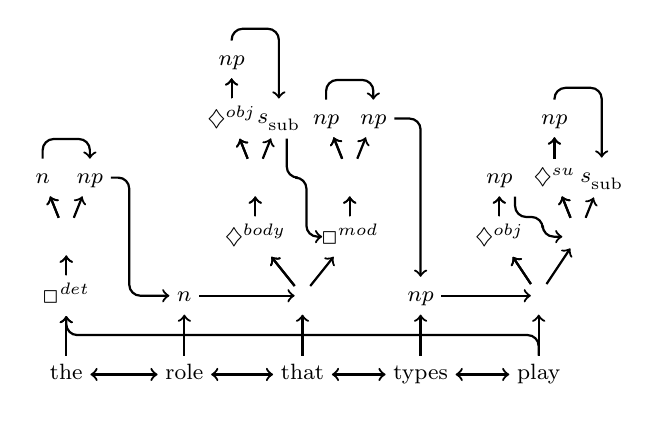
\begin{tikzpicture}
        [tree/.style={dashed},
         ctx/.style={thick, ->, rounded corners},
         ctxbi/.style={thick, <->}]
        \tikzset{every node/.style={outer sep=0pt}}
        	\smaller
        		\node			(w1)				at (-8.5, 0)  		{\hnorm the};
        		\node			(t1_det)			at (-8.5, 1)		{\hnorm $\Box^{det}$};
        		\node			(t1_li)				at (-8.5, 1.75)		{\hnorm $\li$};
        		\node			(t1_n)				at (-8.8, 2.5)		{\hnorm $n$};
        		\node			(t1_np)				at (-8.2, 2.5)		{\hnorm $np$};
        		\node			(w2)				at (-7,0)			{\hnorm role};
        		\node			(t2_n)				at (-7, 1)			{\hnorm $n$};
        		\node			(w3)				at (-5.5, 0)		{\hnorm that};
        		\node			(t3_li1)			at (-5.5, 1)		{\hnorm $\li$};
        		\node			(t3_rc)				at (-6.1, 1.75)		{\hnorm $\diamondsuit^{body}$};
        		\node			(t3_mod)			at (-4.9, 1.75)		{\hnorm $\Box^{mod}$};
        		\node			(t3_li2)			at (-6.1, 2.5)		{\hnorm $\li$};
        		\node			(t3_li3)			at (-4.9, 2.5)		{\hnorm $\li$};
        		\node			(t3_obj)			at (-6.4, 3.25)		{\hnorm $\diamondsuit^{obj}$};
        		\node			(t3_np)			at (-6.4, 4)		{\hnorm $np$};
        		\node			(t3_ss)				at (-5.8, 3.25)		{\hnorm $\ssub$};
        		\node			(t3_np1)			at (-5.2, 3.25)		{\hnorm $np$};
        		\node			(t3_np2)			at (-4.6, 3.25)		{\hnorm $np$};
        		\node			(w4)				at (-4, 0)			{\hnorm types};
        		\node			(t4_np)				at (-4, 1)			{\hnorm $np$};
        		\node			(w5)				at (-2.5, 0)		{\hnorm play};
        		\node			(t5_li1)			at (-2.5, 1)		{\hnorm $\li$};
        		\node			(t5_obj)			at (-3, 1.75)		{\hnorm $\diamondsuit^{obj}$};
        		\node			(t5_np1)			at (-3, 2.5)		{\hnorm $np$};
        		\node			(t5_li2)			at (-2, 1.75)		{\hnorm $\li$};
        		\node			(t5_su)				at (-2.3, 2.5)		{\hnorm $\diamondsuit^{su}$	};
        		\node			(t5_np2)				at (-2.3, 3.25)		{\hnorm $np$};
        		\node			(t5_ss)				at (-1.7, 2.5)		{\hnorm $\ssub$};
				%%%% Tree Structure
				\draw[tree]		(t1_det) -- (t1_li) -- (t1_n);
				\draw[tree] 	(t1_li)	-- (t1_np);
				\draw[tree]		(t3_li1) -- (t3_rc) -- (t3_li2) -- (t3_obj) -- (t3_np);
				\draw[tree] 	(t3_li2) -- (t3_ss);
				\draw[tree]		(t3_li1) -- (t3_mod) -- (t3_li3) -- (t3_np1);
				\draw[tree]		(t3_li3) -- (t3_np2);
				\draw[tree]		(t5_li1) -- (t5_obj) -- (t5_np1);
				\draw[tree]		(t5_li1) -- (t5_li2) -- (t5_su) -- (t5_np2);
				\draw[tree]		(t5_li2) -- (t5_ss);
        		%
        		\visible<2->{
        			\draw[ctxbi] (w1) -- (w2);
        			\draw[ctxbi] (w2) -- (w3);
        			\draw[ctxbi] (w3) -- (w4);
        			\draw[ctxbi] (w4) -- (w5);
        		}
        		\visible<3-8>{
        			\draw[ctx] ($(w5.north)$) |- (-4, 0.5) -| ($(t1_det.south)$);
        			\visible<4->{
					\draw[ctx] (t1_det) -- (t1_li);
					}
					\visible<5->{
					\draw[ctx] (t1_li) -- (t1_n);
					}
					\visible<6->{
					\draw[ctx] ($(t1_n.north)$) -- ($(t1_n.north) + (0, 0.25)$) -| ($(t1_np.north)$);
					}
					\visible<7->{
					\draw[ctx] ($(t1_np.east)$) -- ($(t1_np) + (0.5, 0)$) |- ($(t2_n.west)$);
					}
					\visible<8->{
					\draw[ctx] (t2_n) -- (t3_li1);
					\draw[ctx] (t3_li1) -- (t3_rc);
					\draw[ctx] (t3_rc) -- (t3_li2);
					\draw[ctx] (t3_li2) -- (t3_obj);
					\draw[ctx] (t3_obj) -- (t3_np);
					\draw[ctx] ($(t3_np.north)$) -- ($(t3_np.north) + (0, 0.15)$) -| ($(t3_ss.north)$);
					\draw[ctx] ($(t3_ss.south) + (0.1, 0)$) |- ($(-5.45, 2.5)$) -- ($(-5.45, 1.75)$) -- ($(-5.25, 1.75)$);
					\draw[ctx] (t3_mod) -- (t3_li3);
					\draw[ctx] (t3_li3) -- (t3_np1);
					\draw[ctx] ($(t3_np1.north)$) -- ($(t3_np1.north) + (0, 0.25)$) -| ($(t3_np2.north)$);
					\draw[ctx] ($(t3_np2.east)$) -| ($(t4_np.north)$);
					\draw[ctx] (t4_np) -- (t5_li1);
					\draw[ctx] (t5_li1) -- (t5_obj);
					\draw[ctx] (t5_obj) -- (t5_np1);
					\draw[ctx] ($(t5_np1.south) + (0.2, 0)$) |- ($(-2.45, 2)$) -- ($(-2.45, 1.75)$) -- ($(-2.2, 1.75)$);
					\draw[ctx] (t5_li2) -- (t5_su);
					\draw[ctx] (t5_su) -- (t5_np2);
					\draw[ctx] ($(t5_np2.north)$) -- ($(t5_np2.north) + (0, 0.15)$) -| ($(t5_ss.north)$);
        			}
        		}
        		\visible<10->{
        			\draw[ctx] (w1) -- (t1_det);
        			\draw[ctx] (w2) -- (t2_n);
        			\draw[ctx] (w3) -- (t3_li1);
        			\draw[ctx] (w4) -- (t4_np);
        			\draw[ctx] (w5) -- (t5_li1);
					\visible<11->{
						\draw[ctx] (t1_det) -- (t1_li);
						\draw[ctx] (t3_li1) -- (t3_rc);
						\draw[ctx] (t3_li1) -- (t3_mod);
						\draw[ctx] (t5_li1) -- (t5_obj);
						\draw[ctx] (t5_li1) -- (t5_li2);
						\visible<12->{
							\draw[ctx] (t1_li) -- (t1_n);
							\draw[ctx] (t1_li) -- (t1_np);
							\draw[ctx] (t3_rc) -- (t3_li2);
							\draw[ctx] (t3_mod) -- (t3_li3);
							\draw[ctx] (t5_obj) -- (t5_np1);
							\draw[ctx] (t5_li2) -- (t5_su);
							\draw[ctx] (t5_li2) -- (t5_ss);
							\draw[ctx] (t3_li2) -- (t3_obj);
							\draw[ctx] (t3_li2) -- (t3_ss);
							\draw[ctx] (t3_li3) -- (t3_np1);
							\draw[ctx] (t3_li3) -- (t3_np2);
							\draw[ctx] (t5_su) -- (t5_np2);
							\draw[ctx] (t3_obj) -- (t3_np);
						}
					}
				}
        \end{tikzpicture}
\end{frame}


\section{Geometry}

\begin{frame}{Post-modernity}
    \smaller
    neither sequence nor tree but \alert{sequence of trees}
    
    $
    p(\sigma_1, \dots \sigma_m ~ | ~ w_1, \dots w_n) \approx \prod_i^m (\sigma_i~|~\sigma_j : \mathrm{depth}(\sigma_j) < \mathrm{depth}(\sigma_i), w_1,\dots w_n)$\\
    \vfill
    
    	     \centering
        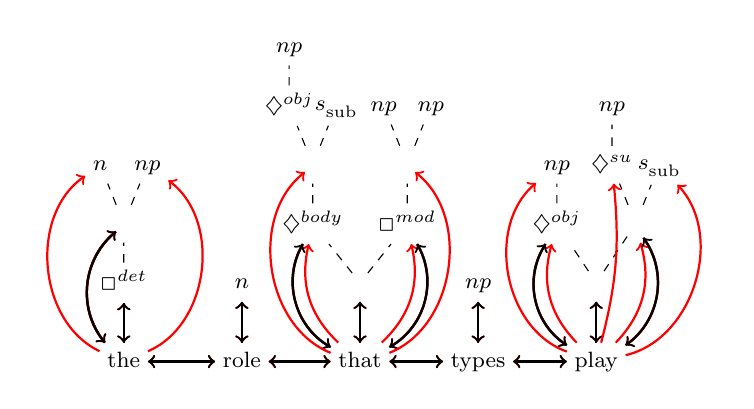
\begin{tikzpicture}
        [state/.style={},
        tree/.style={dashed},
        ctx/.style={thick, ->, rounded corners},
        rctx/.style={thick, <-, rounded corners},
        actx/.style={ctx, red},
        arctx/.style={rctx, red},
        ctxbi/.style={thick, <->},
        actxbi/.style={ctxbi,red}]
        \tikzset{every node/.style={outer sep=0pt}}
        	\smaller
        		\node			(w1)				at (-8.5, 0)  		{\hnorm the};
        		\node			(t1_det)			at (-8.5, 1)			{\hnorm $\Box^{det}$};
        		\node			(t1_li)			at (-8.5, 1.75)		{\hnorm $\li$};
        		\node			(t1_n)			at (-8.8, 2.5)		{\hnorm $n$};
        		\node			(t1_np)			at (-8.2, 2.5)		{\hnorm $np$};
        		\node			(w2)				at (-7,0)			{\hnorm role};
        		\node			(t2_n)			at (-7, 1)			{\hnorm $n$};
        		\node			(w3)				at (-5.5, 0)			{\hnorm that};
        		\node			(t3_li1)			at (-5.5, 1)			{\hnorm $\li$};
        		\node			(t3_rc)			at (-6.1, 1.75)		{\hnorm $\diamondsuit^{body}$};
        		\node			(t3_mod)			at (-4.9, 1.75)		{\hnorm $\Box^{mod}$};
        		\node			(t3_li2)			at (-6.1, 2.5)		{\hnorm $\li$};
        		\node			(t3_li3)			at (-4.9, 2.5)		{\hnorm $\li$};
        		\node			(t3_obj)			at (-6.4, 3.25)		{\hnorm $\diamondsuit^{obj}$};
        		\node			(t3_np)			at (-6.4, 4)			{\hnorm $np$};
        		\node			(t3_ss)			at (-5.8, 3.25)		{\hnorm $\ssub$};
        		\node			(t3_np1)			at (-5.2, 3.25)		{\hnorm $np$};
        		\node			(t3_np2)			at (-4.6, 3.25)		{\hnorm $np$};
        		\node			(w4)				at (-4, 0)			{\hnorm types};
        		\node			(t4_np)			at (-4, 1)			{\hnorm $np$};
        		\node			(w5)				at (-2.5, 0)			{\hnorm play};
        		\node			(t5_li1)			at (-2.5, 1)			{\hnorm $\li$};
        		\node			(t5_obj)			at (-3, 1.75)		{\hnorm $\diamondsuit^{obj}$};
        		\node			(t5_np1)			at (-3, 2.5)			{\hnorm $np$};
        		\node			(t5_li2)			at (-2, 1.75)		{\hnorm $\li$};
        		\node			(t5_su)			at (-2.3, 2.5)		{\hnorm $\diamondsuit^{su}$	};
        		\node			(t5_np2)			at (-2.3, 3.25)		{\hnorm $np$};
        		\node			(t5_ss)			at (-1.7, 2.5)		{\hnorm $\ssub$};
				%%%% Tree Structure
				\draw[tree]		(t1_det) -- (t1_li) -- (t1_n);
				\draw[tree] 		(t1_li)	-- (t1_np);
				\draw[tree]		(t3_li1) -- (t3_rc) -- (t3_li2) -- (t3_obj) -- (t3_np);
				\draw[tree] 		(t3_li2) -- (t3_ss);
				\draw[tree]		(t3_li1) -- (t3_mod) -- (t3_li3) -- (t3_np1);
				\draw[tree]		(t3_li3) -- (t3_np2);
				\draw[tree]		(t5_li1) -- (t5_obj) -- (t5_np1);
				\draw[tree]		(t5_li1) -- (t5_li2) -- (t5_su) -- (t5_np2);
				\draw[tree]		(t5_li2) -- (t5_ss);
        		%
        		\alt<4,7>{
      				\draw[actxbi] (w1) -- (w2);
	      			\draw[actxbi] (w2) -- (w3);
    				\draw[actxbi] (w3) -- (w4);
    				\draw[actxbi] (w4) -- (w5);
       			}
      			{   
       				\draw[ctxbi] (w1) -- (w2);
	       			\draw[ctxbi] (w2) -- (w3);
  					\draw[ctxbi] (w3) -- (w4);
   					\draw[ctxbi] (w4) -- (w5);
       			}
        		\visible<2->{
        			\alt<2>{
		        		\draw[actx] (w1) -- (t1_det);
	    	    		\draw[actx] (w2) -- (t2_n);
	        			\draw[actx] (w3) -- (t3_li1);
	        			\draw[actx] (w4) -- (t4_np);
	        			\draw[actx] (w5) -- (t5_li1);
        			}
        			{\invisible<3>{
		        		\draw[ctx] (w1) -- (t1_det);
	    	    		\draw[ctx] (w2) -- (t2_n);
	        			\draw[ctx] (w3) -- (t3_li1);
	        			\draw[ctx] (w4) -- (t4_np);
	        			\draw[ctx] (w5) -- (t5_li1);
        			}}
        		}
        		\visible<3->{
        			\alt<3>{
		        		\draw[arctx] (w1) -- (t1_det);
	    	    		\draw[arctx] (w2) -- (t2_n);
	        			\draw[arctx] (w3) -- (t3_li1);
	        			\draw[arctx] (w4) -- (t4_np);
	        			\draw[arctx] (w5) -- (t5_li1);
        			}
        			{
		        		\draw[rctx] (w1) -- (t1_det);
	    	    		\draw[rctx] (w2) -- (t2_n);
	        			\draw[rctx] (w3) -- (t3_li1);
	        			\draw[rctx] (w4) -- (t4_np);
	        			\draw[rctx] (w5) -- (t5_li1);
        			}
        		}
        		\visible<5->{
        			\alt<5>{
        				\draw[actx] (w1) to[bend left=45] (t1_li);
        				\draw[actx] (w3) to[bend left=30] (t3_rc);
        				\draw[actx] (w3) to[bend right=30] (t3_mod);
						\draw[actx] (w5) to[bend left=30] (t5_obj);
						\draw[actx] (w5) to[bend right=30] (t5_li2);
        			}
        			{\invisible<6>{
    	   				\draw[ctx] (w1) to[bend left=45] (t1_li);
        				\draw[ctx] (w3) to[bend left=45] (t3_rc);
        				\draw[ctx] (w3) to[bend right=45] (t3_mod);
						\draw[ctx] (w5) to[bend left=45] (t5_obj);
						\draw[ctx] (w5) to[bend right=45] (t5_li2);
        			}}
        		}
				\visible<6->{
        			\alt<6>{
        				\draw[arctx] (w1) to[bend left=45] (t1_li);
        				\draw[arctx] (w3) to[bend left=45] (t3_rc);
        				\draw[arctx] (w3) to[bend right=45] (t3_mod);
					\draw[arctx] (w5) to[bend left=45] (t5_obj);
					\draw[arctx] (w5) to[bend right=45] (t5_li2);
        			}
        			{
    	   				\draw[rctx] (w1) to[bend left=45] (t1_li);
        				\draw[rctx] (w3) to[bend left=45] (t3_rc);
        				\draw[rctx] (w3) to[bend right=45] (t3_mod);
					\draw[rctx] (w5) to[bend left=45] (t5_obj);
					\draw[rctx] (w5) to[bend right=45] (t5_li2);
        			}
        		}
        		\visible<8->{
        				\draw[actx] (w1) to[bend left=60] (t1_n);
        				\draw[actx] (w1) to[bend right=60] (t1_np);
        				\draw[actx] (w3) to[bend left=60] (t3_li2);
        				\draw[actx] (w3) to[bend right=60] (t3_li3);
        				\draw[actx] (w5) to[bend left=60] (t5_np1);
        				\draw[actx] (w5) to[bend right=10] (t5_su);
        				\draw[actx] (w5) to[bend right=60] (t5_ss);
        		}
%        		\visible<9->{
%        			\alt<9>{
%        				\draw[arctx] (w1) to[bend left=60] (t1_n);
%        				\draw[arctx] (w1) to[bend right=60] (t1_np);
%        				\draw[arctx] (w3) to[bend left=60] (t3_li2);
%        				\draw[arctx] (w3) to[bend right=60] (t3_li3);
%        				\draw[arctx] (w5) to[bend left=60] (t5_np1);
%        				\draw[arctx] (w5) to[bend right=10] (t5_su);
%        				\draw[arctx] (w5) to[bend right=60] (t5_ss);
%        			}
%        			{
%        				\draw[rctx] (w1) to[bend left=60] (t1_n);
%        				\draw[rctx] (w1) to[bend right=60] (t1_np);
%        				\draw[rctx] (w3) to[bend left=60] (t3_li2);
%        				\draw[rctx] (w3) to[bend right=60] (t3_li3);
%        				\draw[rctx] (w5) to[bend left=60] (t5_np1);
%        				\draw[rctx] (w5) to[bend right=10] (t5_su);
%        				\draw[rctx] (w5) to[bend right=60] (t5_ss);
%        			}
%        		}
        \end{tikzpicture}
        \vfill

		\flushleft
		\textit{(%
			\alt<2->{%
				\alt<2,5,8>{predict}%
				{\alt<3,6>{feedback}{contextualize}}%
			}{encode}%
		)}
\end{frame}

\begin{frame}{Implementation: dynamic graph convolutions}
    \smaller 
    1 decoding step per tree depth; 3 message-passing rounds per step
    \begin{itemize}
        \item \textit{contextualize: states $\to$ states}\\
        \quad \alert{universal transformer encoder w/ relative weights}\\
        \quad (many-to-many, update states with neighborhood context)
        \item \textit{predict: state $\to$ nodes}\\
        \quad \alert{token classification w/ dynamic tree embeddings}\\
        \quad (one-to-many, predict fringe nodes from current state)
        \item \textit{feedback: nodes $\to$ state}\\
        \quad \alert{heterogeneous graph attention}\\
        \quad (many-to-one, update state with last predicted nodes)
    \end{itemize}
\end{frame}

\begin{frame}{Table with numbers}
        \vspace{-10pt}
        \smaller[2]
        \centering
        \begin{tabularx}{0.99\textwidth}{@{}l@{~}L@{}c@{\quad}c@{\quad}c@{\quad}c@{\quad}c@{}}
        & & \multicolumn{5}{c}{\textbf{accuracy} {(\%)}} \\
        \cmidrule(lr){3-7}
        & \multicolumn{1}{c}{\textbf{model}} & {overall} & {frequent} & {uncommon} & {~~rare~~} & {unseen}\\
        \toprule
        \multicolumn{7}{c}{\textit{\textbf{CCGbank} (Combinatory Categorial Grammar, en)}} \\
        \rowcolor{gray!20}
        & Sequential RNN            & 95.10 & 95.48 & 65.76 & 26.02 & 0.00\\
        & Tree Recursive            & 96.09 & 96.44 & 68.10 & \fbox{37.40} & 3.03\\
        % & BERT baseline             & 96.22 & 96.58 & 70.29 & 23.17 & -- \\
        \rowcolor{gray!20}
        & Attentive Convolutions    & 96.25 & \fbox{96.64} & 71.04 & --   & -- \\
        & \textit{this work}         & \fbox{96.29} & 96.61 & \fbox{72.06} & 34.45 & \fbox{4.55}\\
        \addlinespace
        \multicolumn{7}{c}{\textit{\textbf{CCGrebank} (ditto, improved version)}}\\
        \rowcolor{gray!20}
        & Sequential RNN            & 94.44 & 94.93 & 66.90 & 27.41 & 1.23\\
        & Tree Recursive            & 94.70 & 95.11 & 68.86 & 36.76 & \fbox{4.94}\\
        % & BERT baseline             & 94.83 & 95.27 & 68.86 & 23.99 & --\\
        \rowcolor{gray!20}
        & \textit{this work}        & \fbox{95.07} & \fbox{95.45} & \fbox{71.40} & \fbox{37.19} & 3.70\\
        \addlinespace
        \multicolumn{7}{c}{\textit{\textbf{TLGBank} (Lambek calculus \& control modalities, fr)}}\\
        \rowcolor{gray!20}
        & ELMo LSTM                 & 93.20 & 95.10 & 75.19 & 25.85 & -- \\
        % & BERT baseline             & \fbox{95.93} & \fbox{96.44} & 81.39 & 47.45 & --\\
        % \rowcolor{gray!20}
        & \textit{this work}        & \fbox{95.93} & \fbox{96.40} & \fbox{81.48} & \fbox{55.37} & \fbox{7.26}\\
        \addlinespace
        \multicolumn{7}{c}{\textit{\textbf{\AE thel} (van Benthem calculus \& dependency modalities, nl)}}\\
        \rowcolor{gray!20}
        & Sequential Transformer      & 83.67 & 84.55 & 64.70 & 50.58 & \fbox{24.55}\\
        % & BERT baseline             & 93.52 & \fbox{94.83} & 71.85 & 38.06 & --\\
        % \rowcolor{gray!20}
        & \textit{this work}        & \fbox{93.67} & \fbox{94.72} & \fbox{73.45} & \fbox{53.83} & 15.78\\
        \end{tabularx}
\end{frame}


\begin{frame}{Color coded summary}
	\smaller[2]
	{
    \centering
    \begin{tabularx}{1.05\textwidth}{@{}l@{~~~}c@{~~~}c@{~~~}c@{~~~}c@{}}
    \textit{decoder}					& seq2seq[$t$] 				& seq2seq[$\sigma$]				& 	tree					& dynamic graph\\
    \toprule
    \textit{codomain}					& \dr{fixed}				& \dy{open}						& \dg{constrained}			& \dg{constrained}\\
    \textit{context}						& \dg{left}					& \dg{preorder	(global)}		& \dr{ancestors (local)}	& \dg{levels (global)}\\
    \textit{complexity}					& \dy{\# words}				& \dr{\# symbols} 				& \dg{tree depth}			& \dg{tree depth}\\
    \textit{treeness}					& \dr{ignored}				& \dy{implicit}					& \dg{explicit}				& \dg{explicit}\\
    \textit{sequencess}					& \dg{explicit}				& \dy{misaligned}				& \dr{ignored}				& \dg{explicit}\\
    \textit{search?}						& \dg{\cmark}				& \dg{\cmark}					& \dy{?}				& \dy{\textbf{?}}
    \end{tabularx}
    }
    \vfill
    
	\textbf{legend}
	\begin{itemize}
	\item	\dg{green} = good
	\item	\dy{yellow} = meh
	\item	\dr{red} = bad
	\end{itemize}
\end{frame}


\begin{frame}{Take home messages}
    \smaller 
    \alert{use hammers for nails only}\\
    \vfill
    \alert{sparsity}.. a \textit{friend}?
    \begin{itemize}
        \item more rare cats $\implies$ better acquisition of rare cats
        \item cascading effect on performance
    \end{itemize}
    \vfill
\end{frame}

{\setbeamertemplate{headline}{}
\frame{

\begin{center}
    thanks!    
\end{center}
}}


\end{document}